% Global configuration
\documentclass[12pt,a4paper]{report}
\renewcommand{\baselinestretch}{1.5} % interline
\renewcommand{\familydefault}{\rmdefault} % default font

% Main packages
% Initial config
\usepackage[utf8]{inputenc}
\usepackage{glossaries-extra}

% Title and authors
\title{End of Studies Project}
\author{
    Anis, Benna\\
    \texttt{anis@navoy.io}
}
\date{March 2022}

% Import packages
\usepackage{pdfpages}
\usepackage{natbib}
\usepackage{graphicx}
\usepackage{float}
\usepackage{tabularx}
\usepackage{colortbl}
\usepackage{multirow}
\usepackage{caption}
\usepackage{chngcntr}
\usepackage[hyphens]{url}
\usepackage{listings}
\usepackage{color}
\usepackage{textcomp}
\usepackage[toc,page]{appendix}
\usepackage{ragged2e}
\usepackage{enumitem}
\usepackage[parfill]{parskip} % \medskip and \noindent are not needed. See https://tex.stackexchange.com/a/74173/268270
\usepackage{titlesec}
\usepackage{fancyhdr}
\usepackage[a4paper, footskip=0.5in, tmargin=2in, bmargin=0.75in, headheight=1in]{geometry}
\usepackage[nohints]{minitoc}
\usepackage{longtable}

% DEVONLY:
\usepackage{lipsum} % Lorem ipsum


% Global configuration
% Indent subsection title by adding space before it
% https://www.developpez.net/forums/d1762803/autres-langages/autres-langages/latex/mise-forme/indentation-sections-sous-sections/
\makeatletter
\renewcommand\subsection{\@startsection{subsection}{2}{0.5pc} % order of classification and offset
  {1cm \@plus -1ex \@minus -.2ex} % space that will be added above the title
  {2.3ex \@plus .2ex} % space that will be added below the title. inline if negative
  {\reset@font\large\bfseries}}
\makeatother

% Redefine the chaptermark (chapter title in every page)
\renewcommand{\chaptermark}[1]{\markboth{\fontsize{11}{12}\selectfont \MakeUppercase{Chapter \thechapter: #1}}{}}

% Redefine the chapter title format
\titleformat{\chapter}[display]
{\normalfont\huge\bfseries}{\chaptertitlename\ \thechapter}{20pt}{\Huge}

% Redefine the space before and after the chapter titles
\titlespacing*{\chapter}{0pt}{-50pt}{40pt}


% Glossary for acronyms
\input{./src/components/glossary.tex}

% ------------- Document content ------------- %
\begin{document}

% In-document configuration
% document-specific configuration

% Color palette
\definecolor{primary}{cmyk}{0, 0.23, 0.98, 0.17}
\definecolor{secondary}{cmyk}{0.48, 0.16, 0, 0.61}
\definecolor{listinggray}{gray}{0.9}
\definecolor{lbcolor}{rgb}{0.9,0.9,0.9}

% Global Figure and Table count
\counterwithout{figure}{chapter}
\counterwithout{table}{chapter}

% Chapter name on each page
\pagestyle{fancy}
\lhead{}
\chead{}
\renewcommand{\headrulewidth}{0pt} % Remove the underline
\setlength{\headheight}{15pt}

% Initialize the mini toc at the beginning of each chapter
% More config https://tex.stackexchange.com/a/4858/268270
\dominitoc[n]
\nomtcrule
\setcounter{minitocdepth}{1}

% Code highlighting for supported languages
% https://en.wikibooks.org/wiki/LaTeX/Source_Code_Listings#Supported_languages
\lstset{
  backgroundcolor=\color{lbcolor},
  tabsize=4,
  rulecolor=,
  language=matlab,
  basicstyle=\scriptsize,
  upquote=true,
  aboveskip={1.5\baselineskip},
  columns=fixed,
  showstringspaces=false,
  extendedchars=true,
  breaklines=true,
  prebreak = \raisebox{0ex}[0ex][0ex]{\ensuremath{\hookleftarrow}},
  frame=single,
  showtabs=false,
  showspaces=false,
  showstringspaces=false,
  identifierstyle=\ttfamily,
  keywordstyle=\color[rgb]{0,0,1},
  commentstyle=\color[rgb]{0.133,0.545,0.133},
  stringstyle=\color[rgb]{0.627,0.126,0.941},
}

% Add custom language support for yaml
% https://tex.stackexchange.com/questions/152829/how-can-i-highlight-yaml-code-in-a-pretty-way-with-listings
\newcommand\YAMLcolonstyle{\color{red}\mdseries}
\newcommand\YAMLkeystyle{\color{black}\bfseries}
\newcommand\YAMLvaluestyle{\color{blue}\mdseries}
\makeatletter
\newcommand\language@yaml{yaml}
\expandafter\expandafter\expandafter\lstdefinelanguage
\expandafter{\language@yaml}
{
keywords={true,false,null,y,n},
keywordstyle=\color{darkgray}\bfseries,
basicstyle=\YAMLkeystyle,                                 % assuming a key comes first
sensitive=false,
comment=[l]{\#},
morecomment=[s]{/*}{*/},
commentstyle=\color{purple}\ttfamily,
stringstyle=\YAMLvaluestyle\ttfamily,
moredelim=[l][\color{orange}]{\&},
moredelim=[l][\color{magenta}]{*},
moredelim=**[il][\YAMLcolonstyle{:}\YAMLvaluestyle]{:},   % switch to value style at :
morestring=[b]',
morestring=[b]",
literate =    {---}{{\ProcessThreeDashes}}3
{>}{{\textcolor{red}\textgreater}}1
{|}{{\textcolor{red}\textbar}}1
{\ -\ }{{\mdseries\ -\ }}3,
}
\lst@AddToHook{EveryLine}{\ifx\lst@language\language@yaml\YAMLkeystyle\fi}
\makeatother
\newcommand\ProcessThreeDashes{\llap{\color{cyan}\mdseries-{-}-}}
% Usage example
% \begin{lstlisting}[language=yaml]
%     stages:
%       - test
%       - buildPublish
%       - deploy
% \end{lstlisting}


% Include the cover page
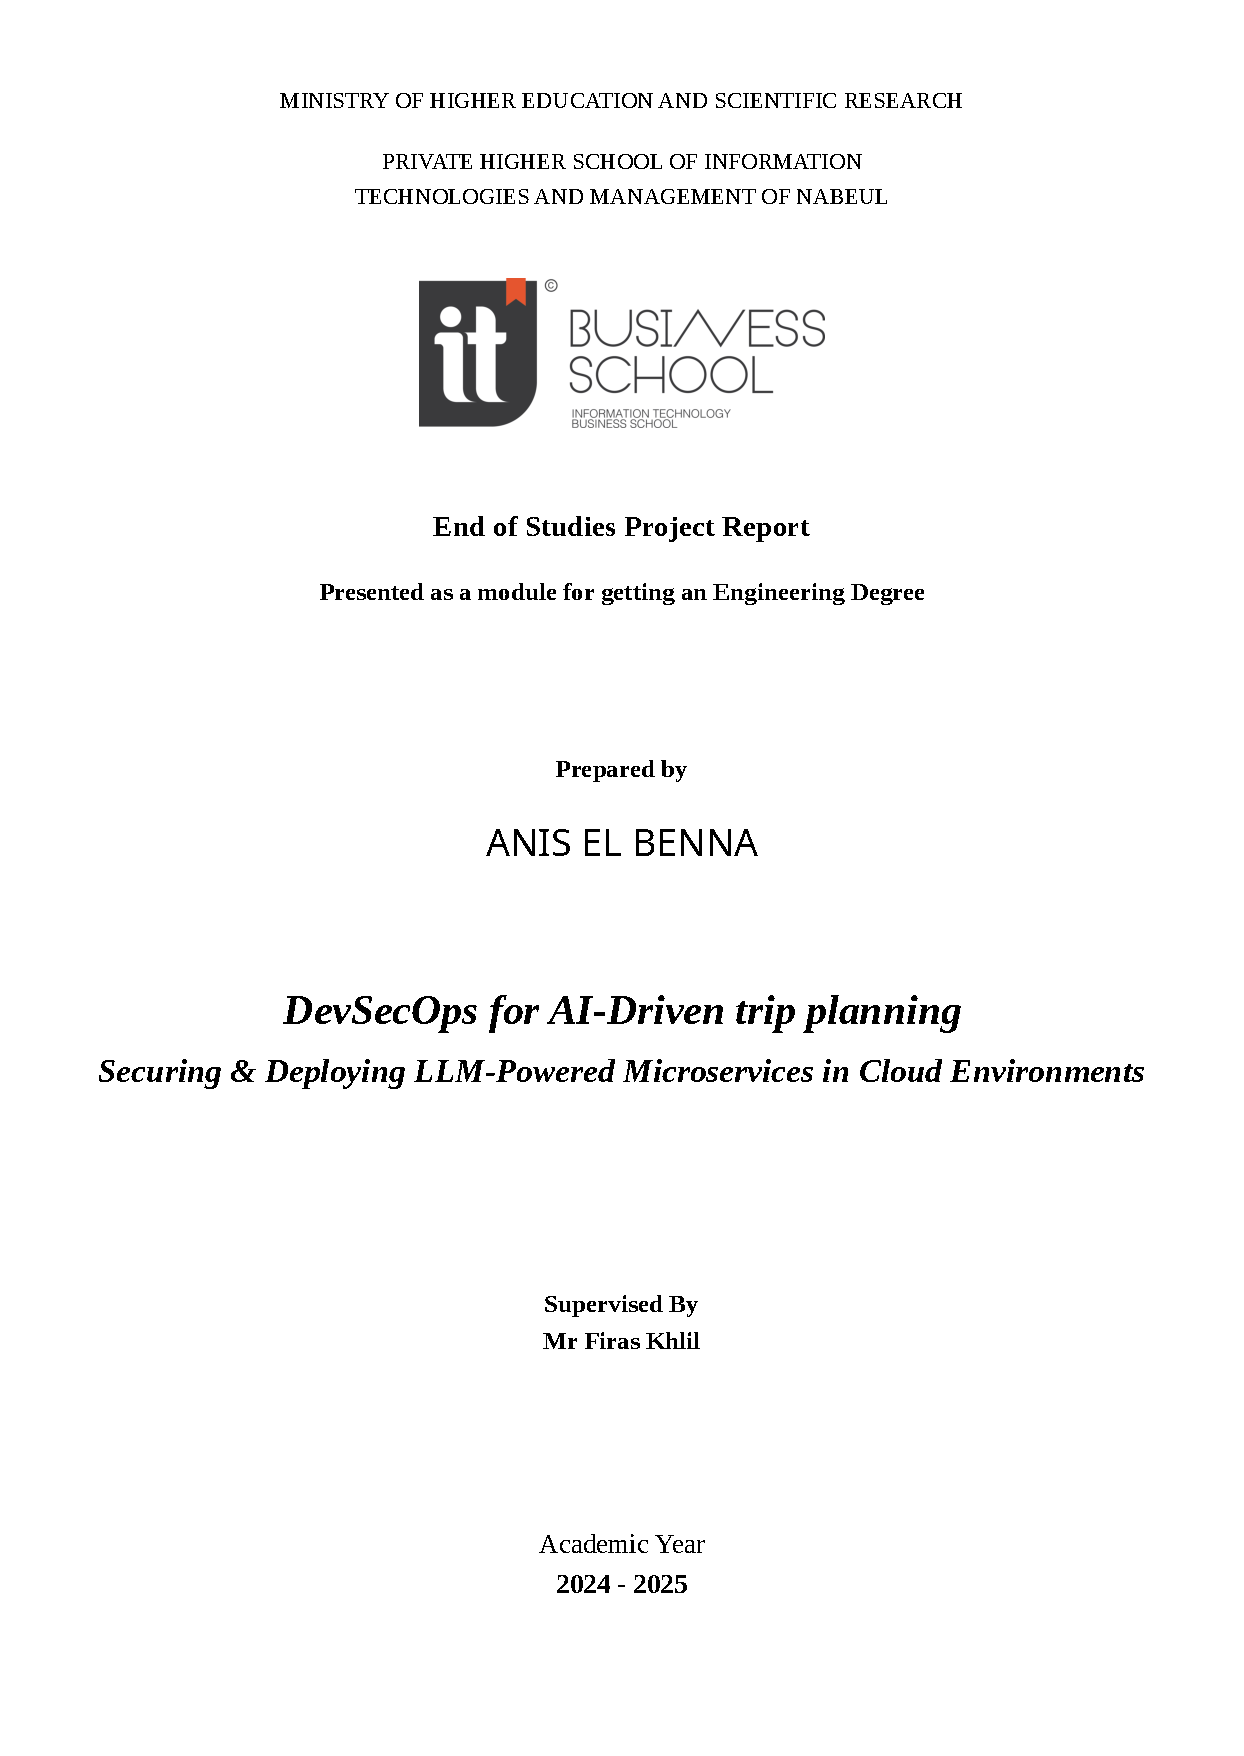
\includepdf[]{./src/assets/pdfs/cover-page.pdf}

% Set page numbering to roman for initial pages
\pagenumbering{roman}
\setcounter{page}{1}

% Dedication and acknowledgments
% \input{src/components/dedications.tex} % Optional
\section*{Acknowledgments}
I would like to take a moment to thank all of those involved in finalizing this work, whether directly or indirectly.

% Thanking the Navoy team
My profound gratitude goes to the entire \textbf{Navoy team} for their warm welcome, invaluable support and for accompanying me throughout this wonderful journey.
Special thanks to the company CEO \textbf{Mr. Haroun Moula} who has been very involved with me almost daily throughout the long period of the internship, his trust in me has truly allowed me to come very far during this project.
I also appreciate my technical supervisor \textbf{Mr. Ala Tabene} for initially showing me the ropes and for his continuous guidance throughout the development process.
My deepest gratefulness also goes to the entire Navoy team for their huge efforts in contributing to making this startup a success, amongst other things, their input has truly been a huge source of knowledge for me and will be forevermore.

% Thanking the University supervisor
I also wish to acknowledge the great support of my university supervisor \textbf{Mr. Firas Khlil} for his assistance, availability and valuable spot-on advice.
His faith in me has truly allowed me to keep working on this project stress-free while confident this report will turn out better than initially intended.

My heartfelt appreciation goes to the jury members who agreed to evaluate my work and I hope they find it up to standard.
I equally thank all of the teachers of the IT Business School
(ITBS) who contributed to my education during these wonderful two and a half years.

\newpage


% Abstract or TL;DR
\section*{Abstract}
The Navoy AI travel platform is a proprietary software solution that enables users to craft and book ultra personalized trips with seamless automated AI flow.
It leverages artificial intelligence to generate highly customized travel itineraries and provides enterprise-level API access for businesses.

To start off, I have two big roles to play.
\textbf{The first} one is to develop new features for the existing AI travel platform while continuously improving the user experience and personalization capabilities.
\textbf{The second} and the most important one is to migrate Navoy from a monolithic application to a \textbf{microservices} architecture in order to make it infinitely scalable. I also have to find the ideal environment to deploy my newly created microservices to, in order to ensure their intra-communication.

I start by breaking the application into various NestJS microservices, build the corresponding docker images then create a shared Helm package for the microservices. Second of all, I setup my own \textbf{self-managed Kubernetes cluster with MicroK8s and ansible scripts}, configure it appropriately to support the specific use-case, then deploy the application stack to both staging and production.

Lastly, using \textbf{GitLab's CI/CD pipelines} and also \textbf{GNU's Makefiles} allows me to automate the whole process from start to finish.
So that in the end, one commit on the main branch is enough to deliver my changes to the clients, which is the standard that \textbf{DevOps compliant} applications should follow.

\newpage


% Print the acronyms list
\printunsrtglossaries
\newpage

% Tables
\renewcommand{\contentsname}{Table of Contents}
\tableofcontents
\listoffigures \mtcaddchapter % https://tex.stackexchange.com/questions/155177/how-to-add-the-word-figure-to-the-list-of-figures
\listoftables \mtcaddchapter % https://tex.stackexchange.com/questions/79869/first-chapter-after-list-of-tables-starts-on-page-2-should-be-1
\clearpage

% Set page numbering to Arabic for main content
\pagenumbering{arabic}

% Include the main app, reset the title spacing for the app chapters only
\titlespacing*{\chapter}{0pt}{20pt}{40pt}
\input{./src/app.tex}
\titlespacing*{\chapter}{0pt}{-50pt}{40pt}

% Generate a webography, for more styles
% see - https://www.overleaf.com/learn/latex/Bibtex_bibliography_styles#Table_of_stylename_values
\renewcommand\bibname{Webography}
\bibliographystyle{unsrt}
\bibliography{references}
\addcontentsline{toc}{chapter}{Webography}
\clearpage

% % Set page numbering to alphabetic for appendices
\pagenumbering{alph}
\setcounter{page}{0}

% Very big diagrams, pictures or schemas go here
% % List of appendices
\begin{appendices}
    % Appendix a
    \section{Azure Network Topology}
    Detailed network topology diagrams for Azure environments.
    \begin{figure}[H]
        \centering
        \makebox[\textwidth]{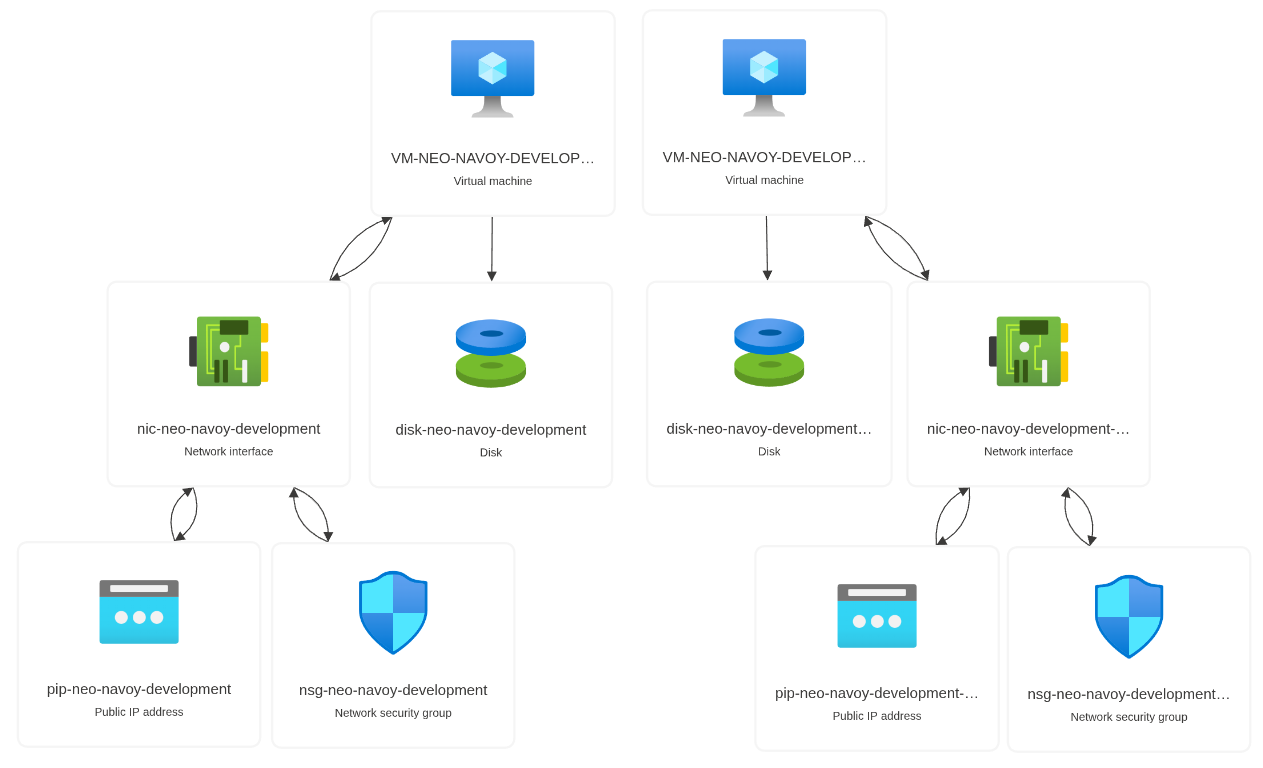
\includegraphics[width=\linewidth]{src/assets/images/azure-development-topology.png}}
        \caption{Azure Development and Alpha Release Topology}
        \label{fig:azure-development-topology-appendix}
    \end{figure}
    \begin{figure}[H]
        \centering
        \makebox[\textwidth]{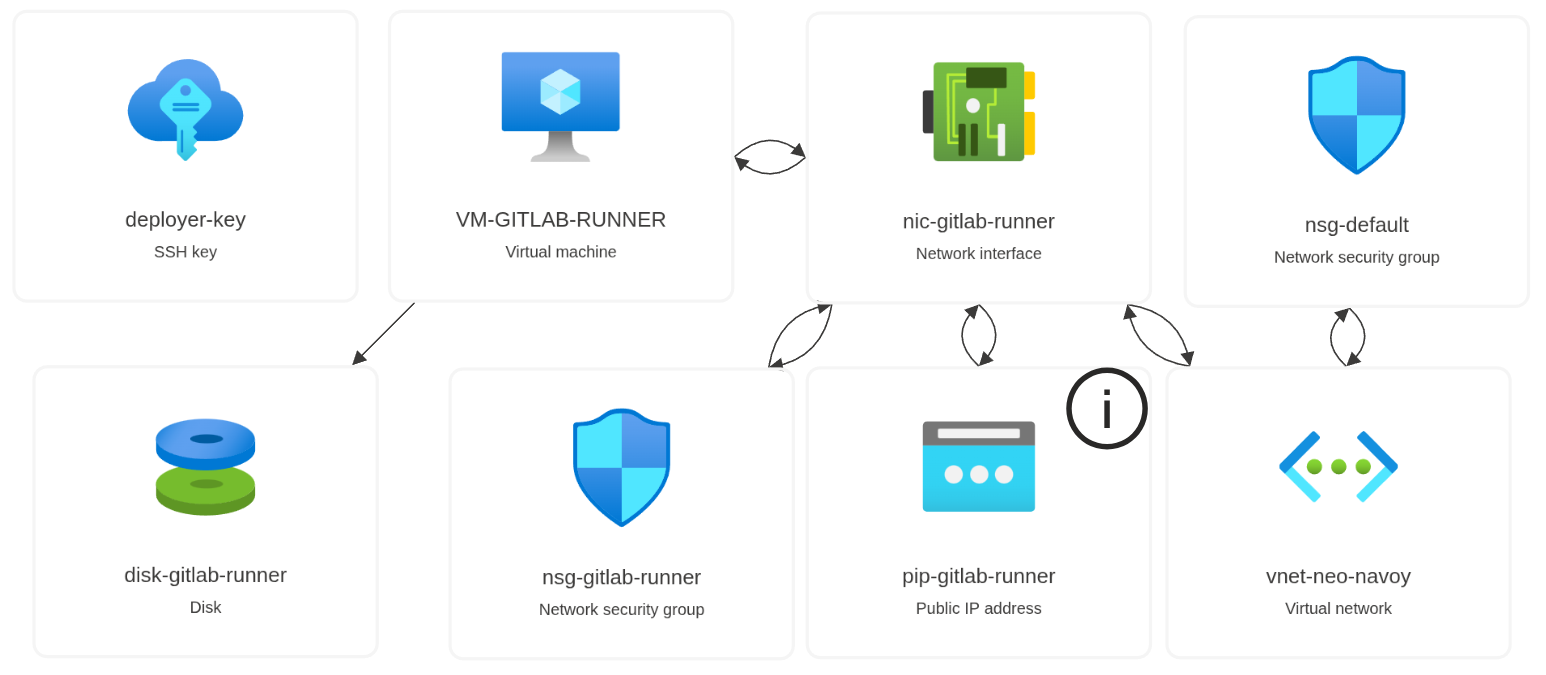
\includegraphics[width=\linewidth]{src/assets/images/azure-shared-topology.png}}
        \caption{Azure Shared Topology}
        \label{fig:azure-shared-topology-appendix}
    \end{figure}
    \newpage

    % Appendix b
    \section{AWS Production Diagram}
    \begin{figure}[H]
        \centering
        \makebox[\textwidth]{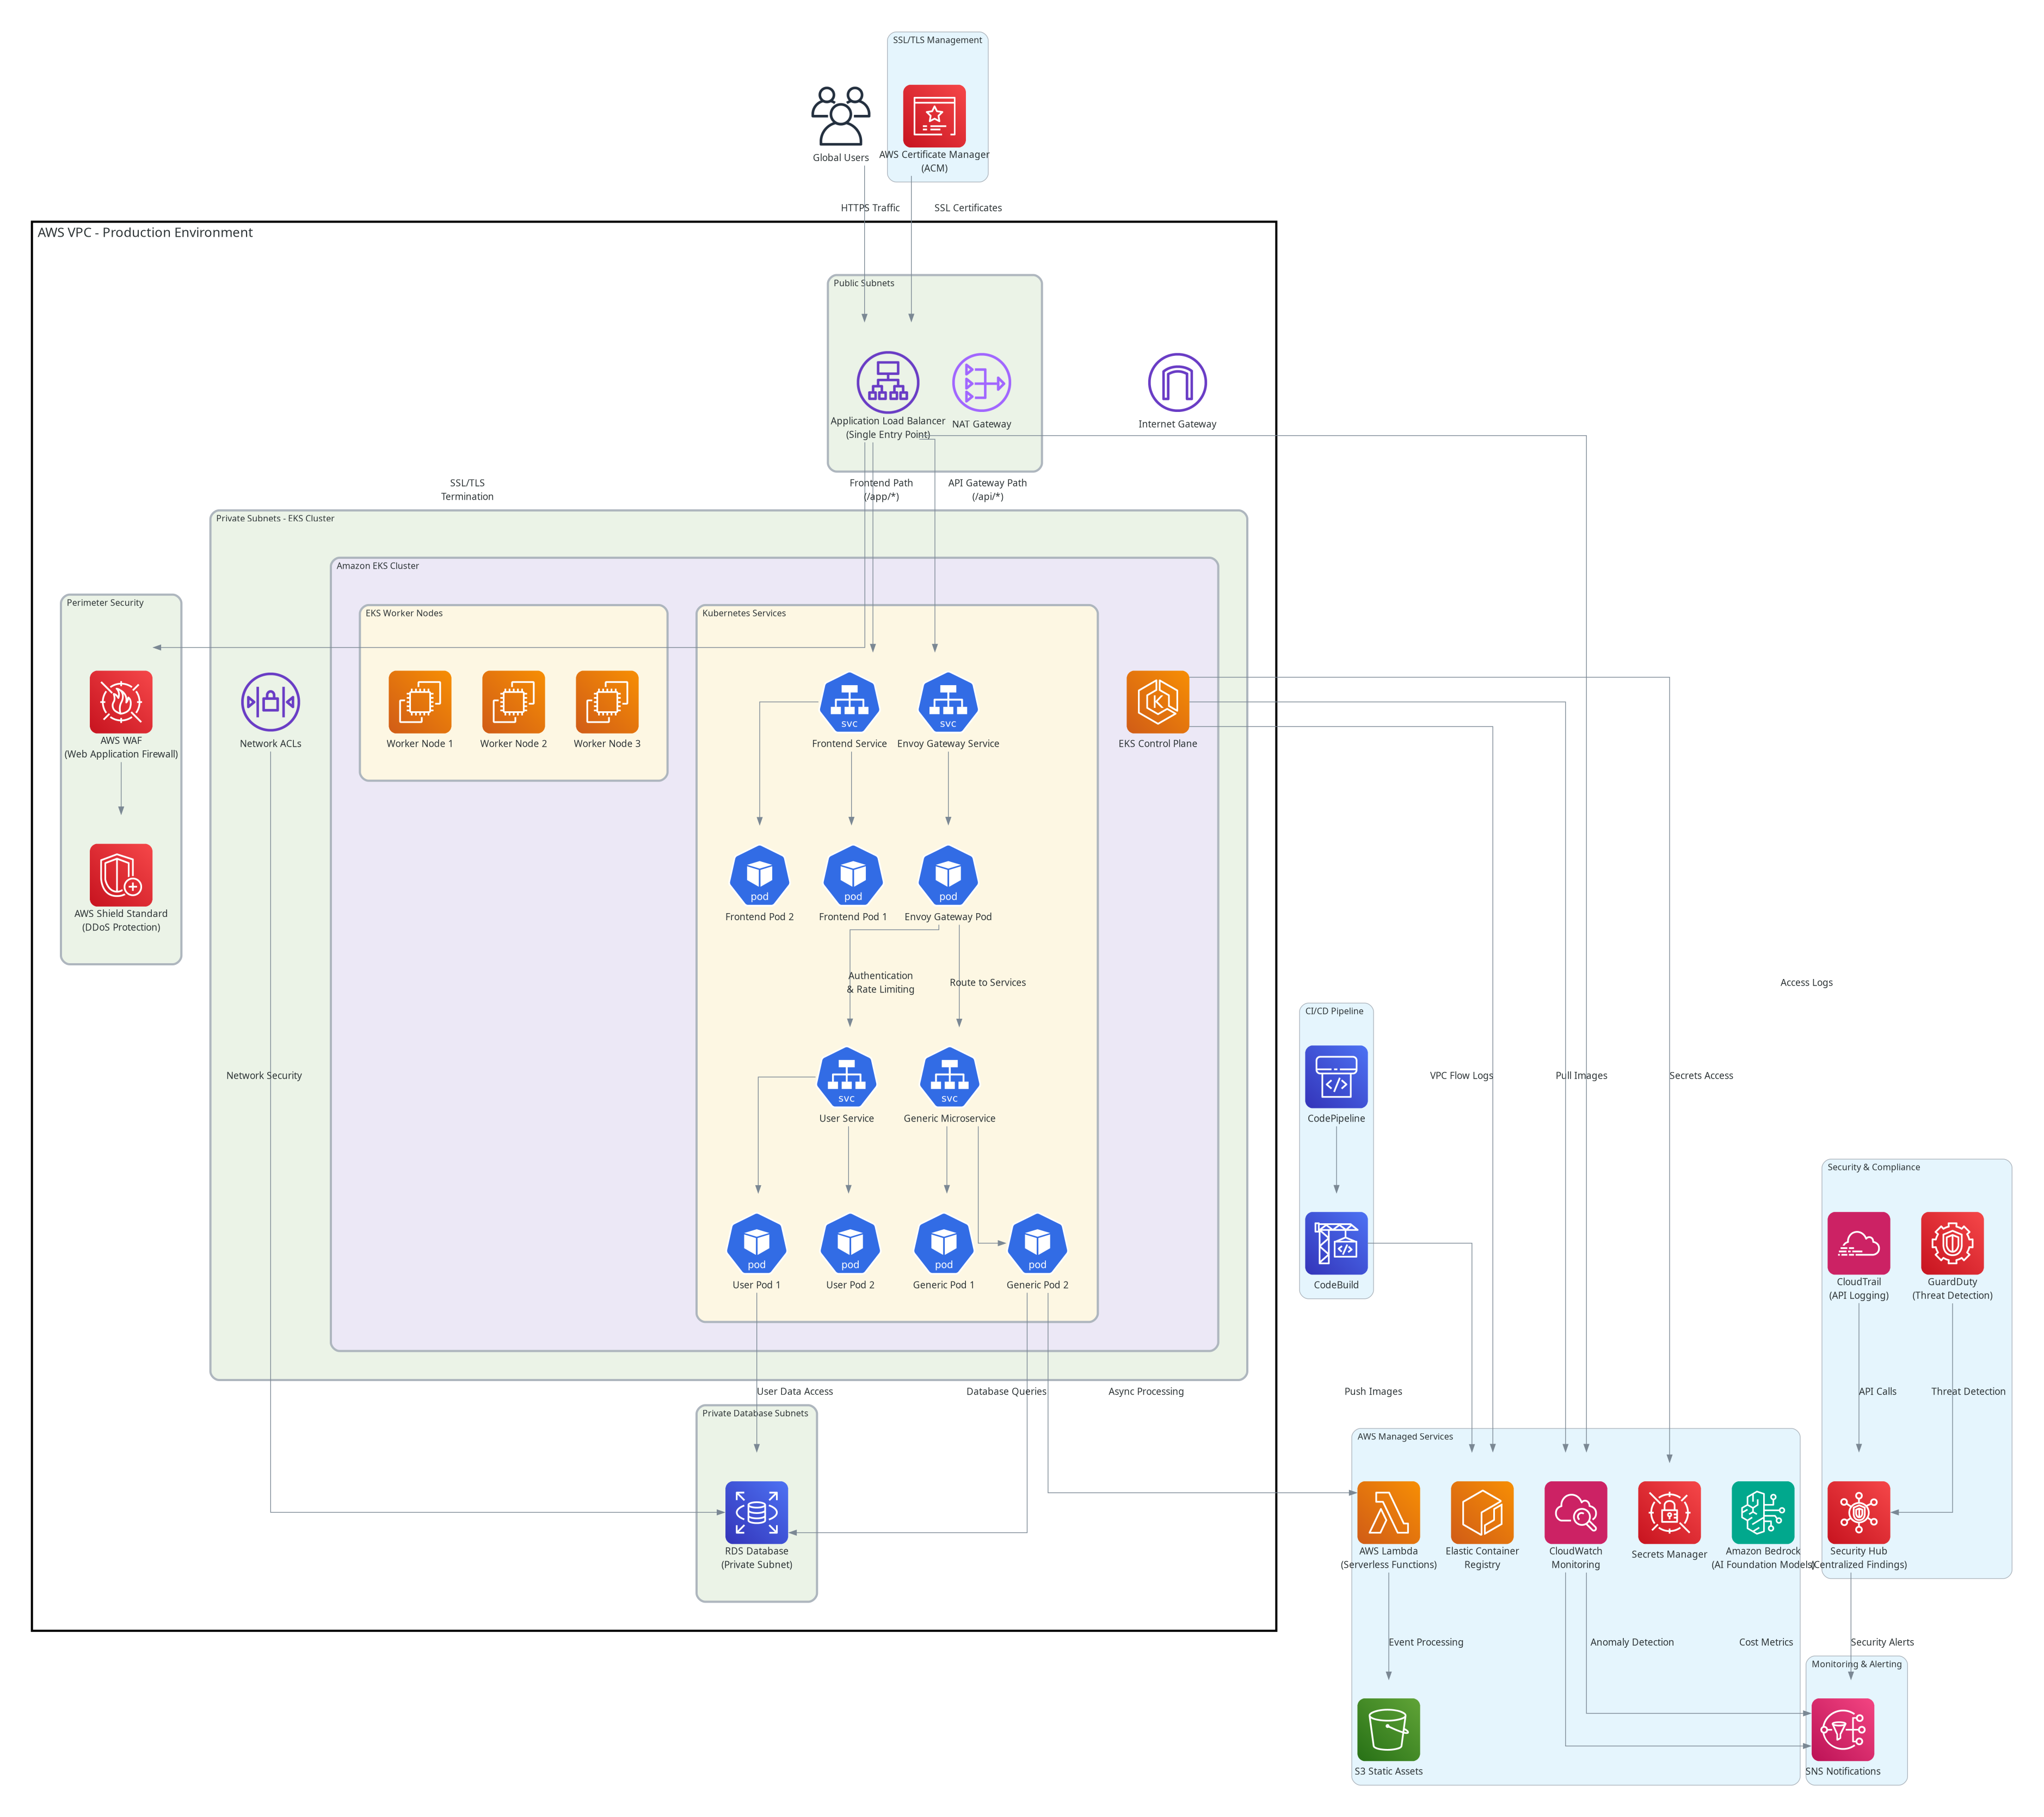
\includegraphics[width=20cm]{src/assets/images/aws-production-architecture.png}}
        \caption{AWS Production Architecture}
        \label{fig:aws-production-architecture-appendix}
    \end{figure}
    \newpage

    % Appendix c
    \section{Overall System Architecture}
    Comprehensive system architecture diagram showing the complete microservices design and inter-service communication patterns.

    \begin{figure}[H]
        \centering
        \makebox[\textwidth]{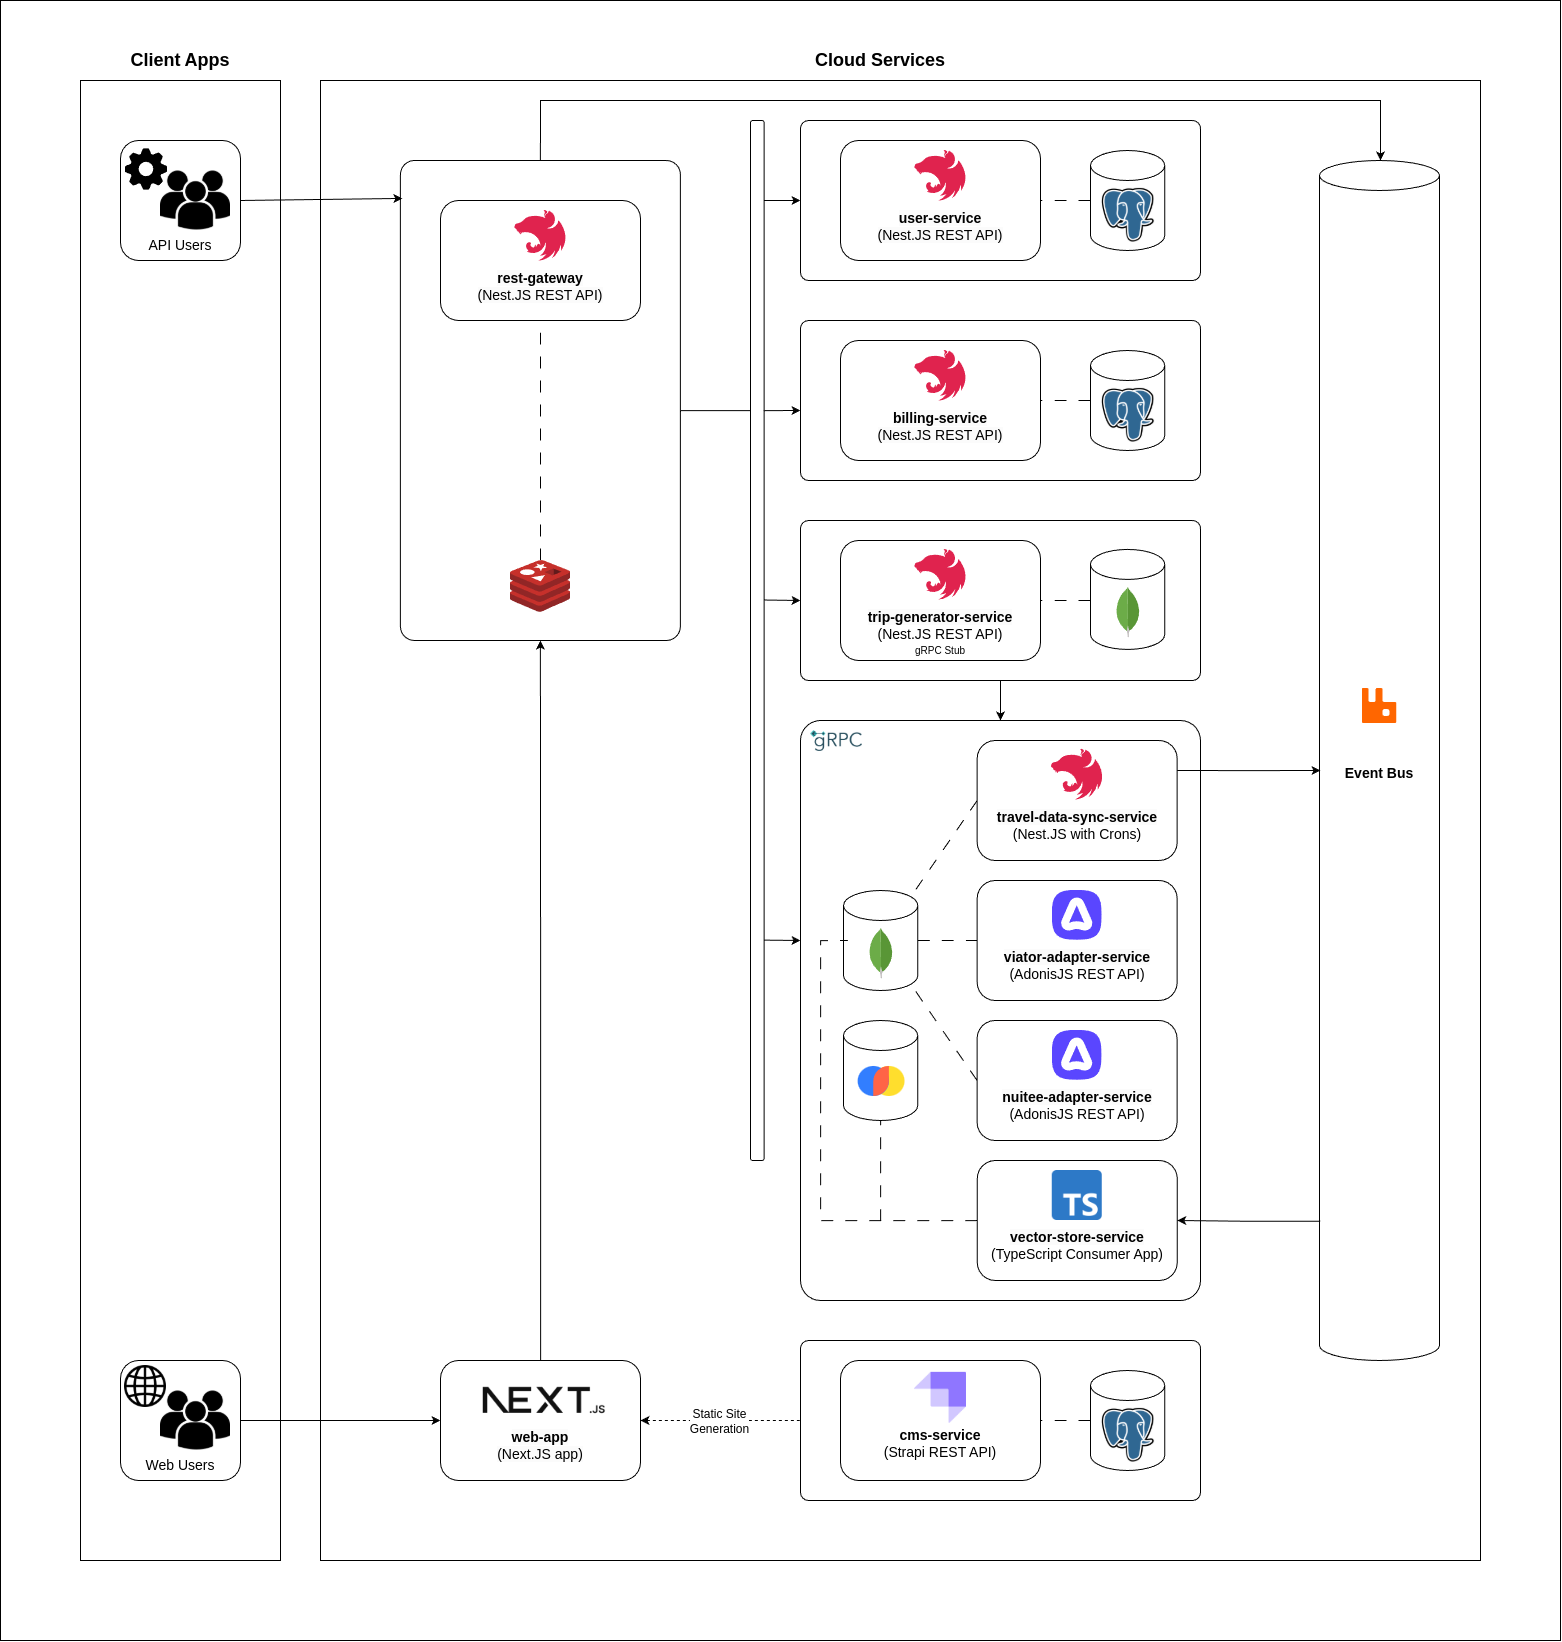
\includegraphics[width=\linewidth]{src/assets/diagrams/software-architecture.drawio.png}}
        \caption{Navoy AI Travel Platform - Complete System Architecture}
        \label{fig:system-architecture-detailed-appendix}
    \end{figure}
    \newpage
\end{appendices}


% Remove page numbering for abstract
\pagenumbering{gobble}

% % Abstract or TL;DR
% \section*{Abstract}
The Navoy AI travel platform is a proprietary software solution that enables users to craft and book ultra personalized trips with seamless automated AI flow.
It leverages artificial intelligence to generate highly customized travel itineraries and provides enterprise-level API access for businesses.

To start off, I have two big roles to play.
\textbf{The first} one is to develop new features for the existing AI travel platform while continuously improving the user experience and personalization capabilities.
\textbf{The second} and the most important one is to migrate Navoy from a monolithic application to a \textbf{microservices} architecture in order to make it infinitely scalable. I also have to find the ideal environment to deploy my newly created microservices to, in order to ensure their intra-communication.

I start by breaking the application into various NestJS microservices, build the corresponding docker images then create a shared Helm package for the microservices. Second of all, I setup my own \textbf{self-managed Kubernetes cluster with MicroK8s and ansible scripts}, configure it appropriately to support the specific use-case, then deploy the application stack to both staging and production.

Lastly, using \textbf{GitLab's CI/CD pipelines} and also \textbf{GNU's Makefiles} allows me to automate the whole process from start to finish.
So that in the end, one commit on the main branch is enough to deliver my changes to the clients, which is the standard that \textbf{DevOps compliant} applications should follow.

\newpage


\end{document}
% ------------- Document content ------------- %
